\documentclass[10pt]{beamer}
\usetheme{jambro}

\title[]{Macroeconomia I - Modelo IS-LM}
\author[]{Paulo Victor da Fonseca}
\date{}

\hypersetup{
    colorlinks = true,
    urlcolor = teal,
    linkcolor = teal    
}
\usepackage[portuguese]{babel}
\usepackage{subfig}
\usepackage{emoji}
\usepackage{hyperref}

\begin{document}

\begin{frame}[plain]
    \titlepage{
        \begin{center}
            \begin{minipage}{0.8\textwidth}
                \centering
            \end{minipage}
        \end{center}}
\end{frame}

\begin{frame}{Sumário}
    \tableofcontents
\end{frame}

\section{Políticas fiscal e monetária no modelo IS-LM tradicional}
\subsection{Introdução}
\begin{frame}{Introdução}
    \begin{itemize}
        \item Vimos, anteriormente, que as políticas fiscal e monetária são as duas principais ferramentas de política macroeconômica às quais o governo pode recorrer na tentativa de manter a economia crescendo a uma taxa razoável, com inflação baixa.
        \bigskip
        \item Elas também são ferramentas de política que o governo utiliza para tentar encurtar as recessões e para evitar que as expansões fujam de controle.
        \bigskip
        \item A política fiscal tem seu impacto inicial no mercado de bens, e a política monetária nos mercados de ativos, principalmente.
        \bigskip
        \item Mas, como os mercados de bens e financeiros estão intimamente interligados, as políticas fiscal e monetária produzem efeitos tanto sobre o nível de produto quanto sobre as taxas de juros.
    \end{itemize}
\end{frame}

\section{Política monetária}
\subsection{Política monetária}
\begin{frame}{Política monetária}
    \begin{itemize}
        \item Vimos que a condução da política é feita, principalmente, por meio de \textcolor{blue}{operações de mercado aberto}.
        \bigskip
        \item Em uma operação de mercado aberto, o Banco Central compra títulos (ou, às vezes, outros ativos) em troca de moeda, elevando, assim, o estoque de moeda em circulação. Ou os vende em troca de moeda paga pelos compradores de títulos, reduzindo, assim, o estoque monetário.
        \bigskip
        \item Quando o BC compra títulos, ele reduz a quantidade disponível no mercado e, assim, tende a aumentar seus preços - ou a reduzir seus rendimentos.
        \bigskip
        \item Somente a uma taxa de juros mais baixa o público estará preparado para reter uma fração menor de sua riqueza na forma de títulos e uma fração maior na forma de moeda.
    \end{itemize}
\end{frame}

\begin{frame}{Política monetária}
\begin{itemize}
    \item Formalmente, os efeitos de uma expansão monetária sobre o nível de produto e as taxas de juros podem ser analisados utilizando o ferramental de estática comparativa.
    \bigskip
    \item As relações IS e LM são dadas por:
    \begin{align}
    Y &= C(Y-T) + I(Y,i) + G, \tag{IS} \\
    \frac{M}{P} &= L(Y,i). \tag{LM}
    \end{align}
    \bigskip
    \item Tomando o diferencial total de primeira ordem, obtemos:
    \begin{align}
        dY &= C_{Y^D} dY - C_{Y^D}T + I_YdY + I_idi + dG, \tag{IS'} \\
        \frac{1}{P}dM - \frac{M}{P^2}dP &= L_YdY + L_idi. \tag{LM'}
    \end{align}
\end{itemize}
\end{frame}

\begin{frame}{Política monetária}
\begin{itemize}
    \item Em termos matriciais, temos:
    \begin{equation}
        \begin{bmatrix}
            1-C_{Y^D}-I_Y & -I_i \\ L_Y & L_i
        \end{bmatrix}\begin{bmatrix}
            dY\\di
        \end{bmatrix} = \begin{bmatrix}
            -C_{Y^D} & 1 & 0 & 0 \\
            0 & 0 & \frac{1}{P} & -\frac{M}{P^2}
        \end{bmatrix}\begin{bmatrix}
            dT \\ dG \\ dM \\ dP
        \end{bmatrix}. \label{eq1} 
    \end{equation}
    \bigskip
    \item Portanto, os multiplicadores de política monetária são dados por:
    \begin{eqnarray}
    \frac{dY}{dM} &=& \frac{I_i/P}{L_i(1-C_{Y^D}-I_Y) + L_YI_i} > 0, \label{eq2} \\
    \frac{di}{dM} &=& \frac{(1-C_{Y^D}-I_Y)/P}{L_i(1-C_{Y^D}-I_Y) + L_YI_i} < 0. \label{eq3}
    \end{eqnarray}
\end{itemize}
\end{frame}

\begin{frame}{Política monetária}
\begin{figure}
    \centering
    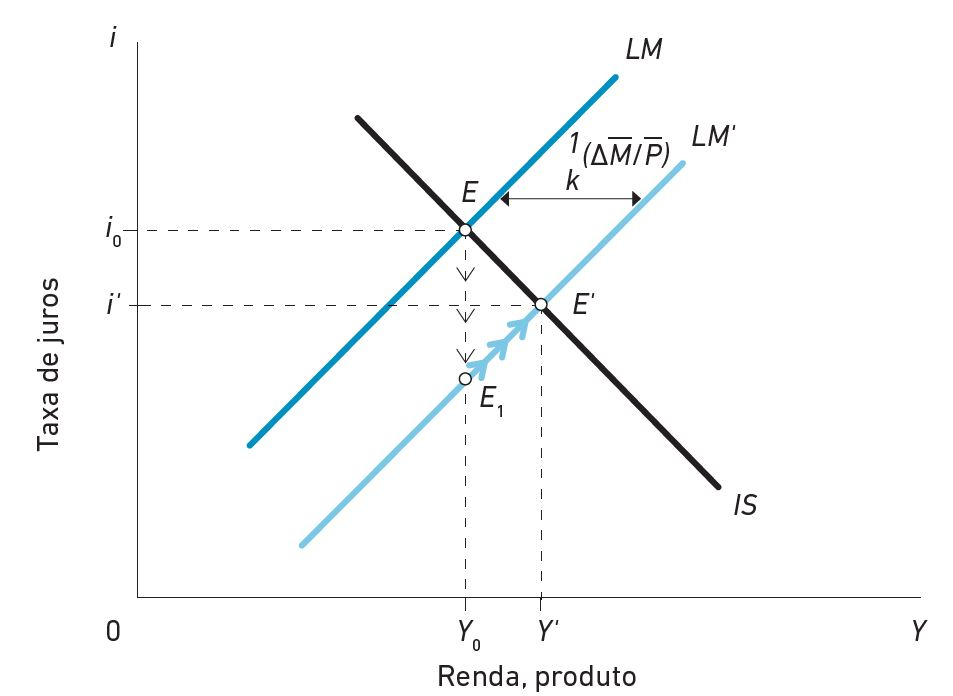
\includegraphics[width=0.6\textwidth]{./figures/aula102_fig1.JPG}
    \caption{Efeitos de uma política monetária expansionista. Fonte: Dornbusch, Fischer e Startz (2013).}
    \label{fig1}
\end{figure}
\end{frame}

\begin{frame}{Política monetária}
\begin{itemize}
    \item Tanto a análise gráfica quanto nossa análise formal nos permitem observar que quanto mais inclinada for a curva LM, maior será a variação no produto agregado.
    \bigskip
    \item Se a demanda por moeda for muito sensível a variações na taxa de juros (LM relativamente plana), uma mudança no estoque monetário pode ser absorvida no mercado de ativos com apenas uma pequena alteração nesta taxa.
    \bigskip
    \item Os efeitos de uma compra no mercado aberto sobre o gasto com investimentos seriam, então, pequenos.
    \bigskip
    \item Por outro lado, se a demanda por moeda não for muito sensível à taxa de juros (LM relativamente inclinada), uma mudança na oferta de moeda irá causar grande variação na taxa de juros e terá efeito considerável sobre a demanda por investimento.
\end{itemize}
\end{frame}

\begin{frame}{Política monetária}
\begin{itemize}
    \item Da mesma forma, se a demanda por moeda for muito sensível à renda, dado aumento no estoque monetário pode ser absorvido com uma mudança relativamente pequena na renda e o multiplicador monetário será menor.
    \bigskip
    \item \textbf{Dinâmica de ajustamento.} O aumento na oferta de moeda cria um excesso de oferta monetária ao qual o público se ajusta ao tentar comprar outros ativos.
    \bigskip
    \item No processo, os preços dos ativos sobem e os rendimentos caem.
    \bigskip
    \item Como os mercados de moeda e de ativos ajustam-se rapidamente, mudamos imediatamente para o ponto $E_1$ na Figura \ref{fig1}, em que o mercado monetário está em equilíbrio e o público está disposto a reter maior quantidade real de moeda, porque a taxa de juros caiu o suficiente.
\end{itemize}
\end{frame}

\begin{frame}{Política monetária}
\begin{itemize}
    \item No ponto $E_1$, no entanto, há excesso de demanda por bens.
    \bigskip
    \item O declínio na taxa de juros, dado o nível inicial de renda, elevou a demanda agregada e está fazendo com que os estoques diminuam.
    \bigskip
    \item Em resposta, o produto se expande e começamos a nos deslocar ao longo da curva LM' para cima.
    \bigskip
    \item Por que a taxa de juros sobe durante o processo de ajuste? Porque o aumento do produto eleva a demanda por moeda e uma demanda maior deve ser compensada por taxas de juros mais altas.
    \bigskip
    \item Portanto, o aumento no estoque monetário inicialmente reduz a taxa de juros, conforme o público ajusta a sua carteira e, depois - como resultado do declínio nas taxas de juros - aumenta a demanda agregada.
\end{itemize}
\end{frame}

\subsection{Mecanismos de transmissão}
\begin{frame}{Mecanismos de transmissão}
    \begin{itemize}
        \item No \textcolor{blue}{mecanismo de transmissão} da política monetária - processo pelo qual as mudanças na política monetária afetam a demanda agregada - duas etapas são essenciais.
        \bigskip
        \item A primeira é que o aumento nos saldos reais gera um desequilíbrio de carteira, ou seja, na taxa de juros e no nível de renda em vigor, as pessoas estão retendo mais moeda do que desejam.
        \bigskip
        \item Isso incentiva os detentores de carteira os detentores de carteira a tentar reduzir suas retenções de moeda por meio da compra de outros ativos, alterando, assim, os preços e rendimentos dos ativos.
        \bigskip
        \item Em outras palavras, a variação na oferta de moeda altera as taxas de juros.
    \end{itemize}
\end{frame}

\begin{frame}{Mecanismos de transmissão}
\begin{itemize}
    \item A Figura \ref{fig2} apresenta um resumo das etapas dos mecanismos de transmissão da política monetária.
\end{itemize}
\bigskip
\begin{figure}
    \centering
    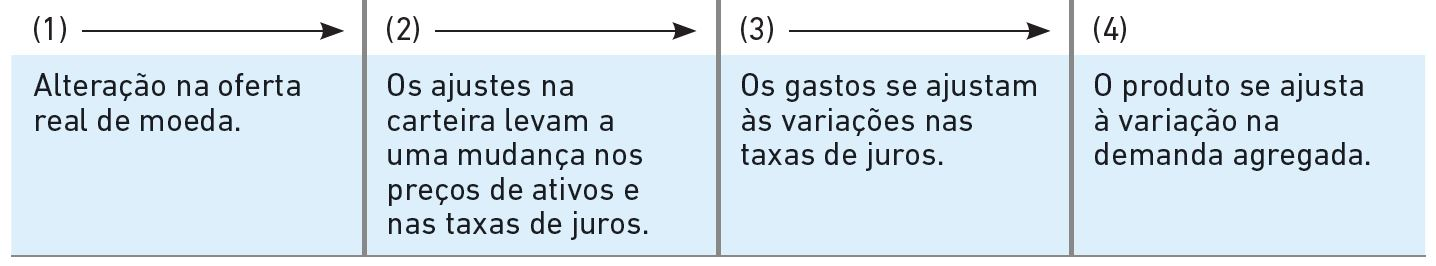
\includegraphics[width=\textwidth]{./figures/aula102_fig2.JPG}
    \caption{Mecanismo de transmissão da política monetária. Fonte: Dornbusch, Fischer e Startz (2013).}
    \label{fig2}
\end{figure}
\end{frame}

\subsection{Armadilha da liquidez}
\begin{frame}{Armadilha da liquidez}
    \begin{itemize}
        \item Um dos casos extremos que vimos ao discutir os efeitos da política monetária sobre a economia é o de \textcolor{blue}{armadilha da liquidez}.
        \bigskip
        \item \textcolor{blue}{Armadilha da liquidez} é uma situação na qual o público está preparado, a uma determinada taxa de juros, para reter qualquer quantidade de moeda que é ofertada.
        \bigskip
        \item Isso implica que a curva LM é horizontal e que variações na quantidade de moeda não a desloquem.
        \bigskip
        \item Neste caso, a política monetária realizada por meio de operações de mercado aberto não tem efeito sobre a taxa de juros ou o nível de renda.
        \bigskip
        \item \textbf{Na armadilha da liquidez, a política monetária é impotente para afetar a taxa de juros}.
    \end{itemize}
\end{frame}

\begin{frame}{Armadilha da liquidez}
\begin{itemize}
    \item A armadilha da liquidez é um instrumento expositivo útil para compreensão das consequências de uma curva LM relativamente plana, mas com pouca relevância para formuladores de políticas econômicas.
    \bigskip
    \item No entanto, uma situação em que a armadilha da liquidez é motivo de fundamental preocupação prática é quando as taxas de juros aproximam-se do \textcolor{blue}{limite inferior da taxa de juros}.
    \bigskip
    \item Nenhuma quantidade de moeda impressa irá reduzir a taxa de juros nominal para abaixo de zero. Por exemplo, a uma taxa de juros negativa de 5\%, poderíamos tomar emprestado \$100 hoje, manter sob forma de moeda e pagar \$95 em um ano e embolsar a diferença. A demanda por moeda seria infinita.
    \bigskip
    \item Uma vez que a taxa de juros chega a zero, não há nada mais que o BC possa fazer com a política monetária \textbf{convencional} para estimular a economia, pois a política monetária não pode reduzir as taxas ainda mais.
\end{itemize}
\end{frame}

\begin{frame}{Armadilha da liquidez}
\begin{figure}
    \centering
    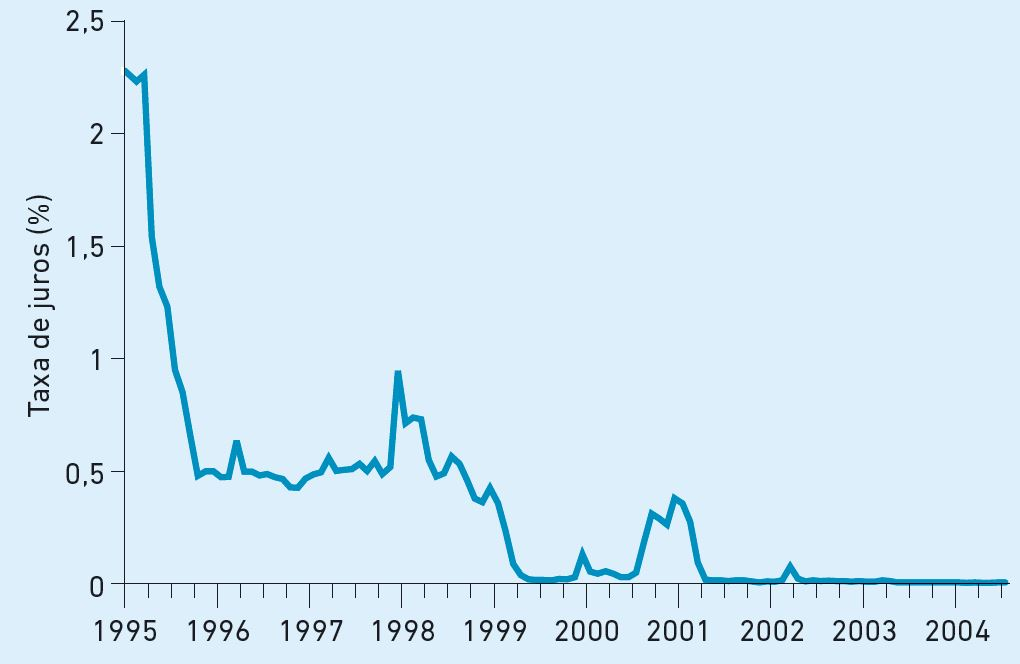
\includegraphics[width=0.7\textwidth]{./figures/aula102_fig3.JPG}
    \caption{Taxas de juros japonesas. Fonte: Dornbusch, Fischer e Startz (2013).}
    \label{fig3}
\end{figure}
\end{frame}

\begin{frame}{Armadilha da liquidez}
\begin{itemize}
    \item Sabemos que a taxa de juros nominal é composta por duas partes: a taxa de juros real e a expectativa de inflação. Formalmente:
    \begin{equation}
        i = r + \pi^e.
        \label{eq4}
    \end{equation}
    \bigskip
    \item Uma economia atinge o limite inferior da taxa de juros quando experimenta uma deflação significativa (deflação significa que os preços estão caindo ou, de forma equivalente, que a taxa de inflação é negativa).
    \bigskip
    \item Uma forma de os formuladores de política econômica evitarem a armadilha da liquidez da taxa de juros no limite inferior é aumentar a oferta de moeda para manter a inflação ligeiramente positiva.
\end{itemize}
\end{frame}

\begin{frame}{Armadilha da liquidez}
\begin{itemize}
    \item Caso uma economia passe por uma armadilha de liquidez com taxa de juros zero, os formuladores de políticas econômicas dos BCs, normalmente, utilizam políticas monetárias \textcolor{blue}{não convencionais}, como comprar títulos de longo prazo, e outros ativos, para injetar moeda na economia.
    \bigskip
    \item \emph{``Para estimular o gasto agregado quando as taxas de juros de curto prazo chegaram a zero, o Fed deve ampliar a escala de suas compras de ativos ou, possivelmente, expandir o menu de ativos que compra. [...] As chances de uma deflação grave nos Estados Unidos parecem remotas, de fato, grande parte devido às forças subjacentes da nossa economia, mas, também devido à determinação do Federal Reserve e de outros formuladores de políticas econômicas do país para agir de forma preventiva contra as pressões deflacionárias.''} (Ben Bernanke em discurso diante do National Economists Club em Washington, 2002)
\end{itemize}
\end{frame}

\begin{frame}{Armadilha da liquidez}
\begin{figure}
    \centering
    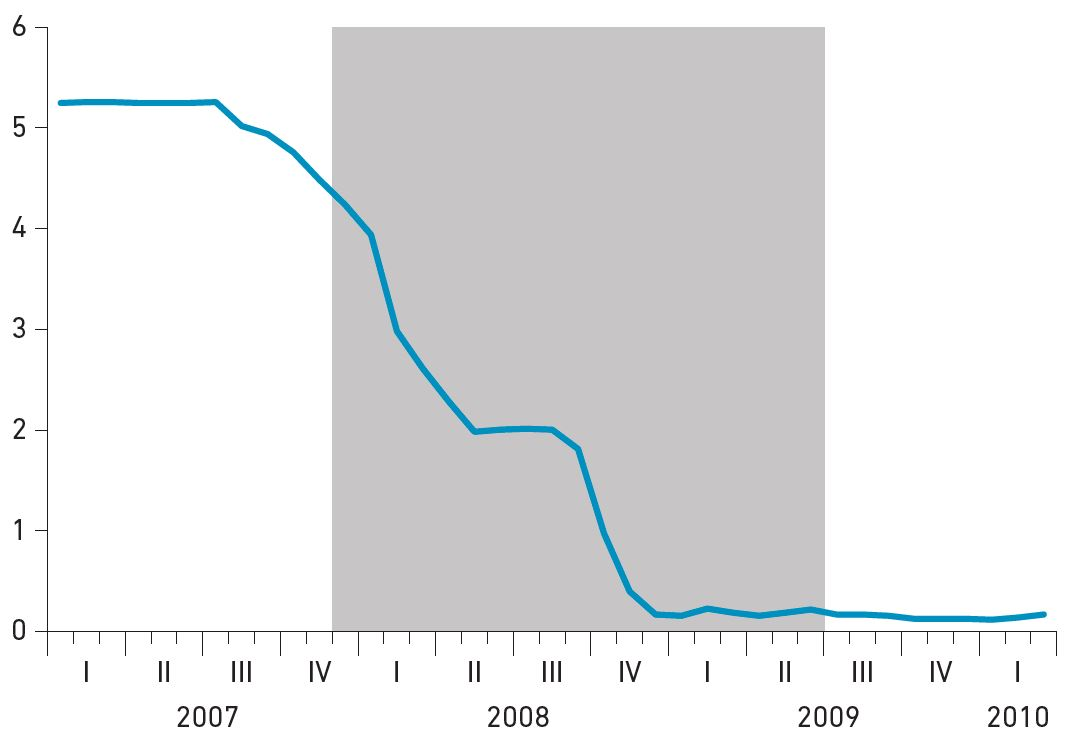
\includegraphics[width=0.7\textwidth]{./figures/aula102_fig4.JPG}
    \caption{Taxas do mercado interbancário (EUA). Fonte: Dornbusch, Fischer e Startz (2013).}
    \label{fig4}
\end{figure}
\end{frame}

\begin{frame}{Armadilha da liquidez}
\begin{itemize}
    \item Quando do discurso de Ben Bernanke em 2002, o argumento era de que uma armadilha da liquidez de taxa de juros no limite inferior era improvável, mas não impossível.
    \bigskip
    \item A Figura \ref{fig4} mostra que com a CFG de 2008, a taxa do mercado interbancário nos EUA tinha de fato atingido o limite inferior no final do ano 2008.
    \bigskip
    \item Isso aconteceu porque o Fed deliberadamente levou a taxa de juros a zero para combater a recessão.
    \bigskip
    \item E assim como Bernanke havia prometido, o Fed comprou ativos não convencionais para conter a crise financeira.
\end{itemize}
\end{frame}

\begin{frame}{Armadilha da liquidez}
\begin{itemize}
    \item Durante a crise, o Fed diminuiu as taxas de juros em 400 centenas de pontos-base.
    \bigskip
    \item Até que ponto o Fed deveria reduzir as taxas de juros para estabilizar a economia? Segundo John Williams, seriam necessárias 400 centenas de pontos-base adicionais. Williams estima que a incapacidade de reduzir as taxas de juros abaixo do limite inferior atrasou a recuperação o suficiente para custar US\$ 1,8 trilhões à economia.
    \bigskip
    \item Com a economia ainda em péssimo estado e sem espaços para reduzir ainda mais a taxa de juros, o Fed realizou uma \textcolor{blue}{flexibilização quantitativa (quantitative easing)} - uma estratégia política de tentar reduzir as taxas de juros de longo prazo por meio da compra de grandes quantidades de ativos financeiros quando a taxa \emph{overnight} é zero.
\end{itemize}
\end{frame}

\begin{frame}[t]{Armadilha da liquidez}
\begin{itemize}
    \item O Fed não comprou apenas letras do Tesouro, mas também uma variedade de outros tipos de dívidas de agências governamentais dos EUA e grandes quantidades de títulos lastreados em hipotecas privadas.
    \bigskip
    \item Durante a recessão, a base monetária mais do que dobrou.
\end{itemize}
\bigskip
\begin{figure}
    \centering
    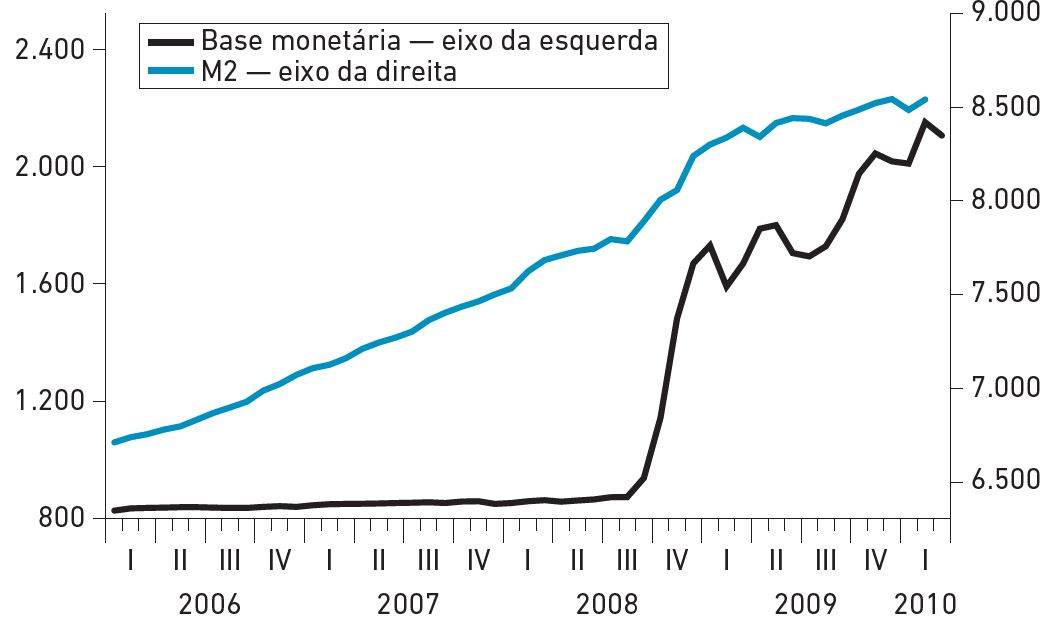
\includegraphics[width=0.5\textwidth]{./figures/aula102_fig5.JPG}
    \caption{Base monetária versus M2. Fonte: Dornbusch, Fischer e Startz (2013).}
    \label{fig5}
\end{figure}
\end{frame}

\begin{frame}{Armadilha da liquidez}
\begin{itemize}
    \item Percebe-se, na Figura \ref{fig5}, que M2 cresceu mais que o habitual, mas nada comparado ao crescimento da base.
    \bigskip
    \item A diferença é uma parte da resposta de como o Fed poderia imprimir enormes quantidades de moeda sem gerar inflação.
    \bigskip
    \item Grande parte do aumento ficou em contas mantidas pelos bancos do Fed sem ser emprestada.
    \bigskip
    \item A segunda razão pela qual o quantitative easing não gerou inflação é que o Fed foi muito explícito de que esperava ``relaxar'' as novas aquisições depois que o perigo para a economia tivesse passado. Assim, \textbf{o aumento da base monetária foi amplamente visto como temporário}.
    \bigskip
    \item Além da flexibilização quantitativa, o Fed realizou a ``flexibilização de crédito'', em que os empréstimos foram direcionados  diretamente aos setores dos mercados financeiros nos quais crédito poderia, basicamente, desaparecer ou tinha de fato desaparecido.
\end{itemize}
\end{frame}

\begin{frame}{Armadilha da liquidez}
\begin{itemize}
    \item Durante a CFG de 2008, as ações monetárias heterodoxas do Fed impediram o que poderia ter sido um colapso indiscriminado dos mercados de crédito, evitando que uma situação muito ruim ficasse ainda pior.
\end{itemize}
\end{frame}

\subsection{Caso clássico}
\begin{frame}{Caso clássico}
    \begin{itemize}
        \item O oposto da curva LM horizontal - política monetária não pode afetar o nível de renda - é a curva LM vertical.
        \bigskip
        \item Como vimos, a curva LM é vertical quando a demanda por moeda é totalmente insensível à taxa de juros.
        \bigskip
        \item Considere uma função de demanda por moeda linear temos, então:
        \begin{equation}
            \frac{\bar{M}}{\bar{P}} = kY - hi.
            \label{eq5}
        \end{equation}
        \bigskip
        \item Se $h = 0$, há um único nível de renda que equilibra o mercado monetário e, portanto, a curva LM é vertical no nível da renda.
    \end{itemize}
\end{frame}

\begin{frame}{Caso clássico}
\begin{figure}
    \centering
    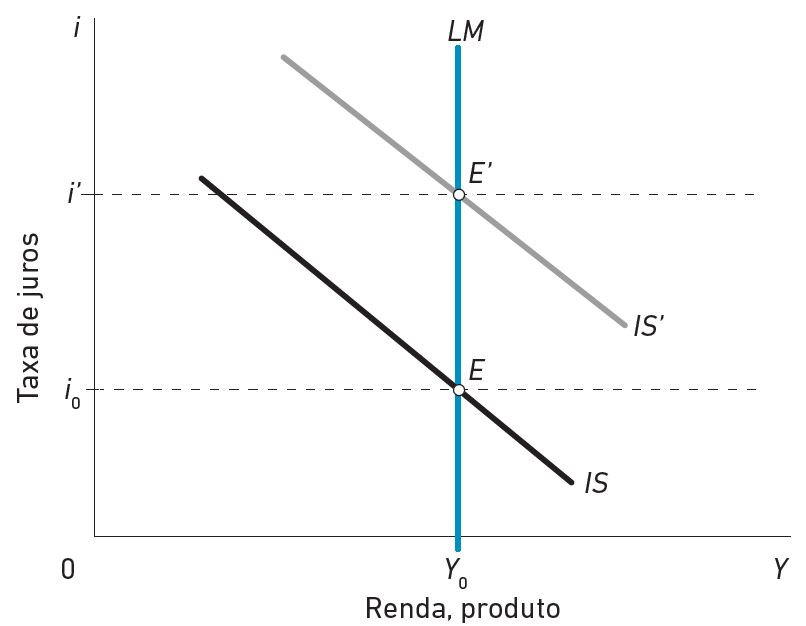
\includegraphics[width=0.6\textwidth]{./figures/aula102_fig6.JPG}
    \caption{Caso clássico. Fonte: Dornbusch, Fischer e Startz (2013).}
    \label{fig6}
\end{figure}
\end{frame}

\begin{frame}{Caso clássico}
\begin{itemize}
    \item A curva LM vertical é chamada de \textcolor{blue}{caso clássico} pois, com $h = 0$, temos a seguinte expressão:
    \begin{equation}
        \bar{M} = k(\bar{P}\times Y). \label{eq6}
    \end{equation}
    \bigskip
    \item Portanto, a renda nominal, $P \times Y$, depende apenas da quantidade de moeda.
    \bigskip
    \item Esta é a clássica \textcolor{blue}{teoria quantitativa da moeda}, que argumenta que o nível de renda nominal é determinado unicamente pela quantidade de moeda.
\end{itemize}
\end{frame}

\begin{frame}{Caso clássico}
\begin{itemize}
    \item Quando a curva LM é vertical, uma mudança na quantidade de moeda tem um efeito máximo sobre o nível de renda.
    \bigskip
    \item Além disso, deslocamentos na curva IS não afetam o nível de renda.
    \bigskip
    \item \textcolor{blue}{Assim, quando a curva LM é vertical, a política monetária tem um efeito máximo sobre o nível de renda e a política fiscal não tem efeito sobre a renda}.
\end{itemize}
\end{frame}

\begin{frame}{Caso clássico}
\begin{itemize}
    \item A curva LM vertical, implicando a eficácia comparativa da política monetária sobre a política fiscal, é por vezes associada à visão de que ``apenas a moeda importa'' para a determinação do produto.
    \bigskip
    \item Como a curva LM é vertical, somente quando a demanda por moeda não depender da taxa de juros a sensibilidade aos juros da demanda acabará por ser uma questão importante na determinação da eficácia de políticas econômicas alternativas.
    \bigskip
    \item No entanto, a evidência empírica sugere que a taxa de juros afeta, sim, a demanda por moeda.
\end{itemize}
\end{frame}

\begin{frame}[t]{Caso clássico}
\begin{itemize}
    \item A Figura \ref{fig7} mostra que, no curto prazo, a elasticidade da demanda com relação à renda real é 0,11 - um aumento de 1\% na renda real aumenta a demanda por moeda em 0,11\%.
    \bigskip
    \item Além disso, um aumento nas taxas de juros reduz a demanda por moeda. Um aumento de 1\% na taxa de juros de curto prazo reduz a demanda por moeda em 0,8\%.
    \bigskip
\end{itemize}
    \begin{figure}
        \centering
        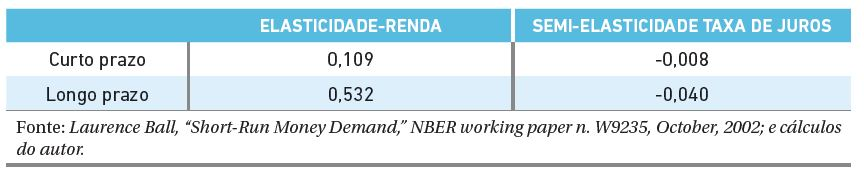
\includegraphics[width=\textwidth]{./figures/aula102_fig7.JPG}
        \caption{Resposta da demanda por moeda M1 real. Fonte: Dornbusch, Fischer e Startz (2013).}
        \label{fig7}
    \end{figure}
\end{frame}

\section{Exercícios}

\begin{frame}[t]{Exercício 1}
    Suponha que a renda nominal das famílias em uma economia seja igual à \$50.000 bilhões e que a demanda por moeda seja dada por:
    \[
    M^d = \$Y(0,2-0,8i).
    \]
    \bigskip
    \begin{enumerate}
        \item Qual é a demanda por moeda quando a taxa de juros é igual à 1\% e 5\%?
        \bigskip
        \item Qual será o impacto sobre a demanda por moeda se a renda nominal declinar em 20\%?
        \bigskip
        \item Qual é a relação entre a demanda por moeda e a renda? Entre demanda por moeda e taxa de juros?
        \bigskip
        \item O que o BC deve fazer com a taxa de juros se deseja aumentar a demanda por moeda?
    \end{enumerate}
\end{frame}

\begin{frame}[t]{Exercício 2}
    Considere um título que promete pagar \$100 em um ano.
    \bigskip
    \begin{enumerate}
        \item Qual é a taxa de juros sobre o título se seu preço hoje é de \$75? \$85? \$95?
        \bigskip
        \item Qual é a relação entre o preço do título e a taxa de juros?
        \bigskip
        \item Se a taxa de juros é de 8\%, qual é o preço do título hoje?
    \end{enumerate}
\end{frame}

\begin{frame}[t]{Exercício 3}
    Suponha as seguintes relações de demanda e oferta de moeda:
    \begin{eqnarray}
    M^s &=& \$8.000 \nonumber \\
    M^d &=& \$40.000(0,25-i) \nonumber
    \end{eqnarray}
    \bigskip
    \begin{enumerate}
        \item Calcule a taxa de juros de equilíbrio.
        \bigskip
        \item Suponha que o BC aumente a taxa de juros de equilíbrio para 10\%, neste caso teremos excesso de oferta de moeda ou excesso de demanda por moeda? Qual política monetária deve ser implementada para atingir a nova taxa de juros de equilíbrio?
    \end{enumerate}
\end{frame}

\begin{frame}[t]{Exercício 4}
    Suponha que a riqueza financeira de um indivíduo é igual à \$50.000 e que sua renda anual seja de \$60.000. Se a função de demanda por moeda for:
    \[
    M^d = \$Y(0,35-i).
    \]
    \bigskip
    \begin{enumerate}
        \item Derive a demanda por títulos deste indivíduo. Suponha que a taxa de juros aumente em 10 pontos percentuais. Qual é o efeito sobre a demanda por títulos?
        \bigskip
        \item Quais os efeitos de um aumento na riqueza sobre a demanda por moeda e na demanda por títulos?
        \bigskip
        \item Quais são os efeitos de um aumento renda sobre a demanda por moeda e sobre a demanda por títulos?
        \bigskip
        \item Considere a seguinte afirmação ``quando as pessoas recebem mais dinheiro, elas obviamente irão deter mais títulos''. O que tem de errado com essa afirmação?
    \end{enumerate}
\end{frame}

\begin{frame}[t]{Exercício 5}
Consideremos o seguinte exemplo numérico do modelo IS-LM:
\begin{eqnarray*}
C &=& 200 + 0,25Y_D \\
I &=& 150 + 0,25Y - 1000i \\
G &=& 250 \\
T &=& 200 \\
\bar{i} &=& 5\%.
\end{eqnarray*}
\begin{enumerate}
    \item Derive a relação IS.
    \bigskip
    \item Qual é o nível de oferta de moeda à meta de taxa de juros estabelecida pelo banco central? Supondo que a função de demanda por moeda seja dada por:
    \[
    \frac{M^d}{P} = 2Y - 8000i.
    \]
    \bigskip
    \item Calcule o consumo, investimento e produto de equilíbrio.
\end{enumerate}
\end{frame}

\begin{frame}[t]{Exercício 5}
    \begin{enumerate}
        \setcounter{enumi}{3}
        \item Suponha que o BC baixe a taxa de juros para 3\%. Como isso muda a curva LM? Resolva para encontrar $Y, I$ e $C$ e descreva os efeitos de uma política monetária expansionista.
        \bigskip
        \item Qual o novo valor de equilíbrio para a oferta de moeda?
        \bigskip
        \item Retorne à situação inicial em que a taxa de juros determinada pelo BC é de 5\%. Se os gastos do governo aumentam para $G = 400$, resuma os efeitos dessa política fiscal expansionista sobre $Y, I$ e $C$? Qual o efeito da política fiscal expansionista sobre a oferta real de moeda?
    \end{enumerate}
\end{frame}

\section{Bibliografia}
\begin{frame}{\emoji{books} Bibliografia}
    \begin{itemize}
        \item BLANCHARD, O. Macroeconomia. 7.ed. São Paulo: Pearson Education do Brasil, 2017\medskip        
        \item DORNBUSCH, R.; FISCHER, S.; STARTZ, R. Macroeconomia. 11.ed. Porto Alegre: AMGH, 2013. Disponível em: \href{https://app.minhabiblioteca.com.br/books/9788580551853}{app.minhabiblioteca.com.br/books/9788580551853}\medskip
        \item FROYEN, R. Macroeconomia: teorias e aplicações. 2.ed. São Paulo: Saraiva, 2013. Disponível em: \href{https://app.minhabiblioteca.com.br/books/9788502175235}{app.minhabiblioteca.com.br/books/9788502175235}\medskip        
    \end{itemize}
\end{frame}
\end{document}